\documentclass[pdf]{beamer}
\mode<presentation>{\usetheme{Warsaw}} 


\usepackage[ddmmyyyy]{datetime}
\renewcommand{\dateseparator}{. }

%\usepackage[backend=biber,style=iso-numeric,autolang=other,bibencoding=utf8,seconds=true]{biblatex}
%\bibliography{../includes/bibliography.bib}

\title{Využitie MS HoloLens 2 vo vzdelávaní} 
\subtitle{Diplomová práca}
\author{Bc. Peter Drábik}
\titlegraphic{
   
\includegraphics[width=3cm]{img/pevs-logo.png}
}

\usepackage[T1]{fontenc}

\begin{document}

\newdate{mydate}{14}{12}{2023}
\date{\displaydate{mydate}}
% Title page frame
\begin{frame}
    \titlepage 
\end{frame}

% Outline frame
\begin{frame}{Obsah}
    \tableofcontents
\end{frame}

\AtBeginSection[]{
    {
        \begin{frame}{Obsah}
        \tableofcontents[currentsection]
        \end{frame}
    }
}

\section{Popis umelej reality}

\subsection{Popis VR}
\begin{frame}{Popis VR}
    \begin{itemize}
        \item Imerzívny zážitok - virtuálne objekty vo virtuálnom prostredí
        \item Headsety doplnené rôznymi controllermi a externými senzormi
    \end{itemize}
    \begin{center}
        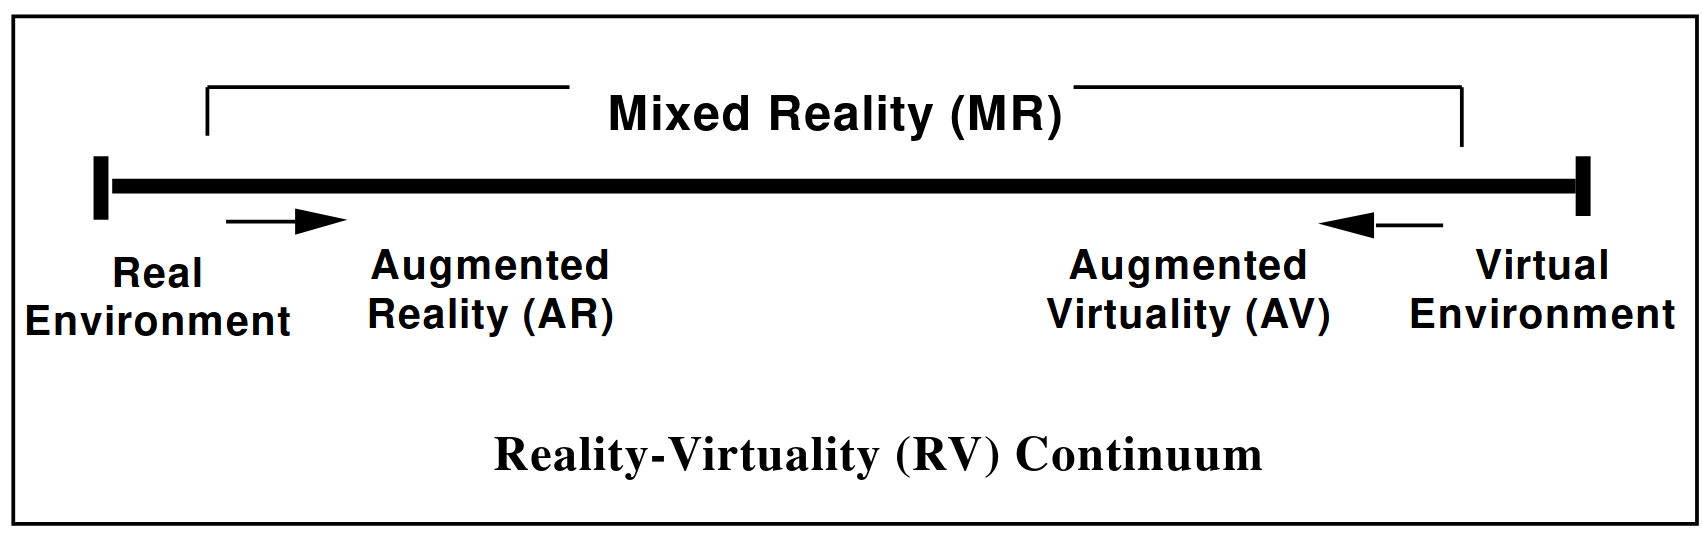
\includegraphics[width=11cm]{../img/continuum.png}
    \end{center}
\end{frame}

\subsection{Popis AR}
\begin{frame}{Popis AR}
    \begin{itemize}
        \item Rozširuje reálne prostredie o virtuálne objekty
        \item Dostupné aj pomocou mobilných telefónov a tabletov
    \end{itemize}
    \begin{center}
        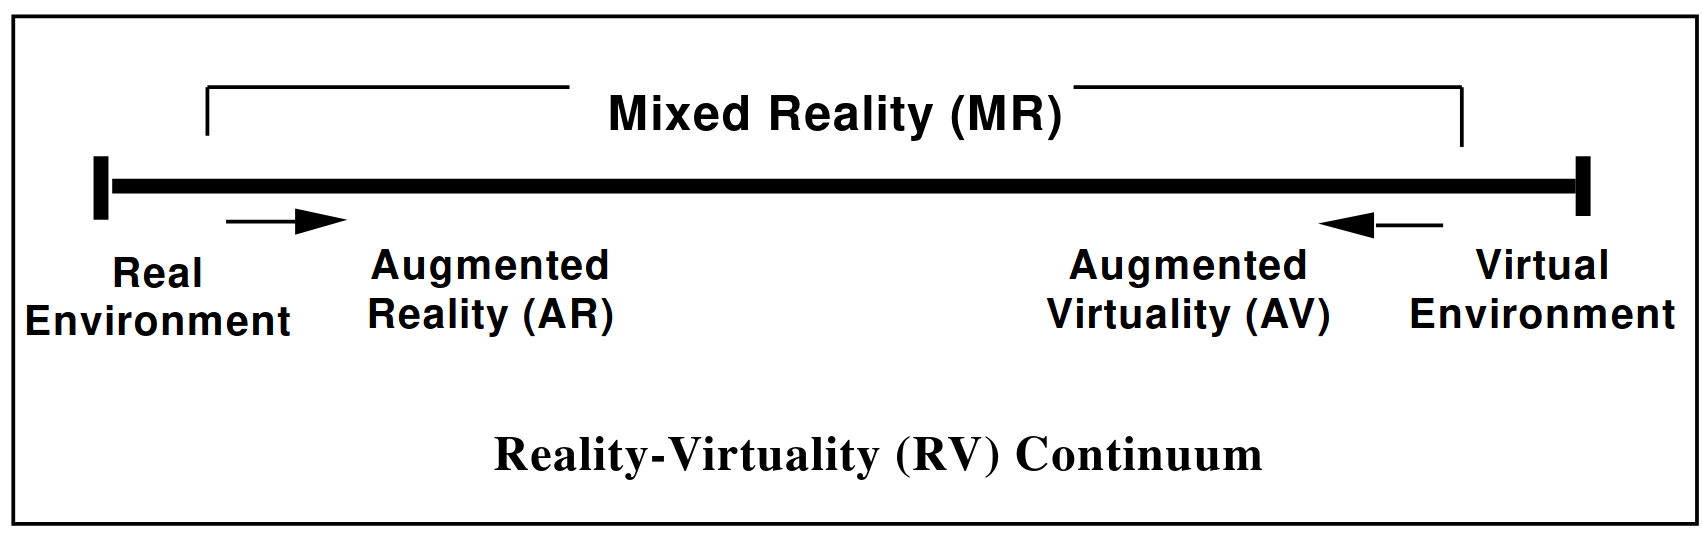
\includegraphics[width=11cm]{../img/continuum.png}
    \end{center} 
\end{frame}

\subsection{Popis MR}
\begin{frame}{Popis MR}
    \begin{itemize}
        \item Kombinuje AR a VR, umožňuje interakciu medzi fyzickými a virtuálnymi objektami
        \item Pokročilé rozpoznávanie fyzického priestoru a umiestňovanie virtuálnych objektov v ňom
    \end{itemize}
    \begin{center}
        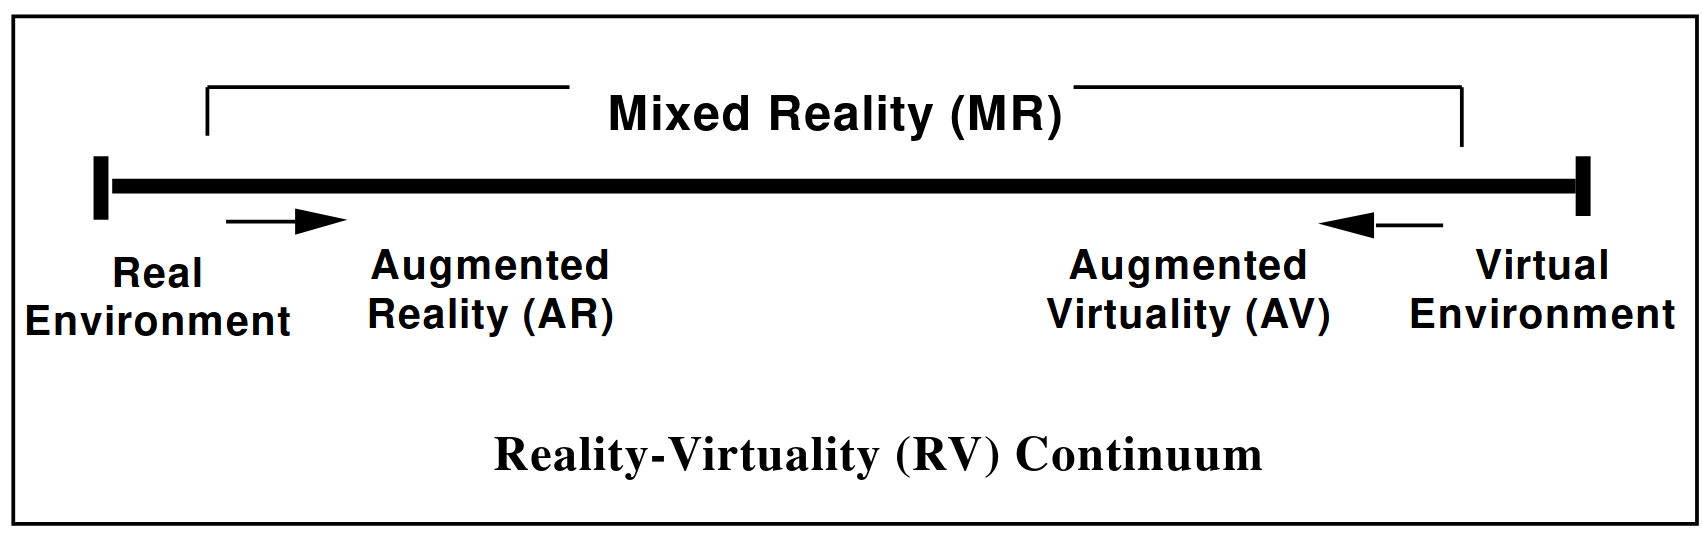
\includegraphics[width=11cm]{../img/continuum.png}
    \end{center} 
\end{frame}

\section{Využitie umelej reality vo vzdelávaní}
\begin{frame}{Využitie umelej reality vo vzdelávaní}
    Závery z rôznych štúdií:
    \begin{itemize}
        \item Umožňuje študentom lepšie sa oboznámiť s komplexnými procesmi v bunke, so štruktúrou bielkovín
        \item Uľahčuje chápanie abstraktných konceptov
        \item Potenciál umelej reality nie je závislý na oblasti vzdelávania ani na charakteristike účastníkov vzdelávacieho procesu
    \end{itemize}
\end{frame}

\section{Problém a jeho riešenie}
\subsection{Identifikované miskoncepcie vo vyučovaní biológie}
\begin{frame}{Identifikované miskoncepcie vo vyučovaní biológie}
    \begin{itemize}
        \item Bunka ako dvojrozmerný objekt \pause
        \item Nepresné analógie používané pri vysvetľovaní princípov šírenia nervového vzruchu
    \end{itemize}
\end{frame}

\subsection{Návrh aplikácie}
\begin{frame}{Návrh aplikácie}
    Kritériá:
        \begin{itemize}
        \item aplikácia bude vyobrazovať trojrozmerný model nervovej bunky,
        \item v rámci aplikácie bude naimplementovaná animácia reprezentujúca zjednodušený model mechanizmu skokového prenosu nervového vzruchu po myelinizovanom vlákne,
        \item na základe používateľského vstupu bude možné túto animáciu opakovane spustiť
        \item rýchlosť tejto animácie bude prispôsobiteľná grafickým ovládacím prvkom.
        \end{itemize}
\end{frame}

\section{Tvorba aplikácie}
\subsection{3D model nervovej bunky}
\begin{frame}{3D model nervovej bunky}
    \begin{itemize}
        \item Použitý nástroj - Blender
        \item 99\% práce - sculpting
    \end{itemize}
\end{frame}

\begin{frame}
    \frametitle{3D model nervovej bunky}    
    \begin{center}
        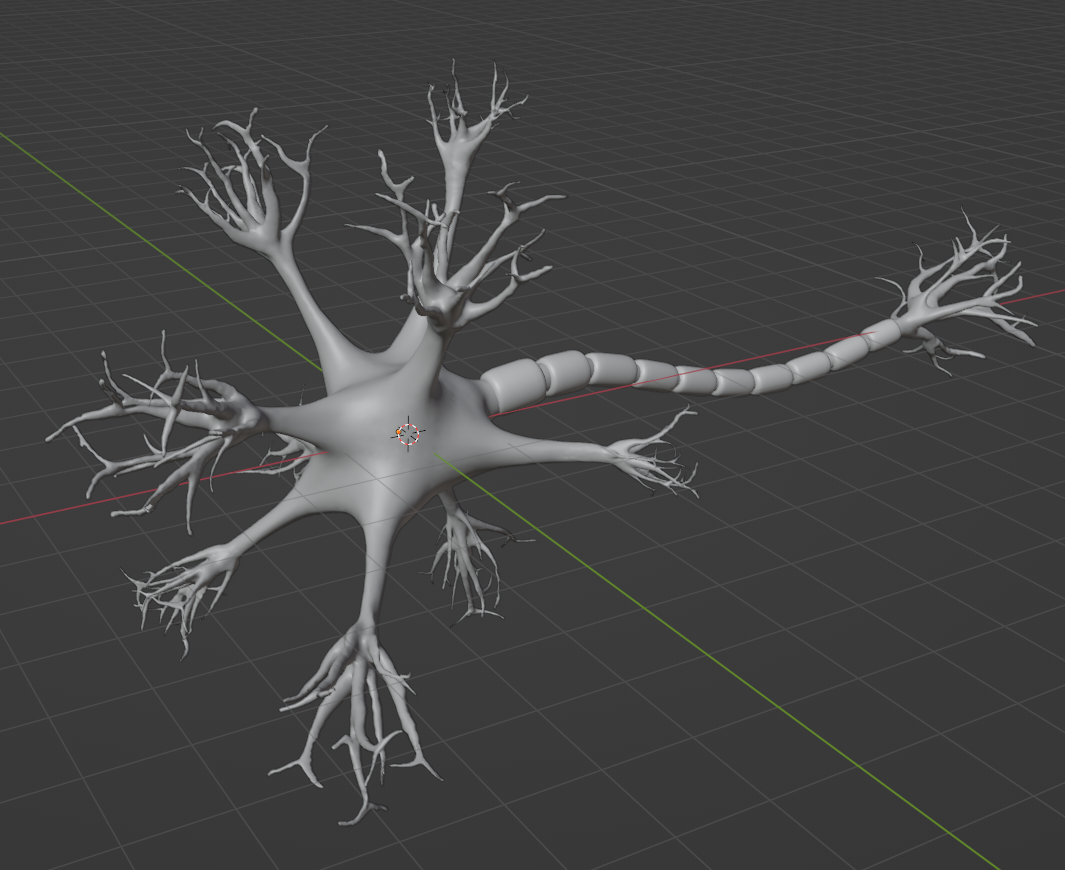
\includegraphics[width=8cm]{../img/finalModel-crop.png}
    \end{center}    
\end{frame}

\subsection{MR aplikácia v Unreal Engine}
\begin{frame}{MR aplikácia v Unreal Engine}
    \begin{itemize}
        \item Unreal Engine - viacúčelový nástroj
        \item Logika aplikácie - Blueprint        
        \item Microsoft Reality Toolkit
    \end{itemize}
\end{frame}

\begin{frame}
    \frametitle{MR aplikácia v Unreal Engine}
    \begin{center}
        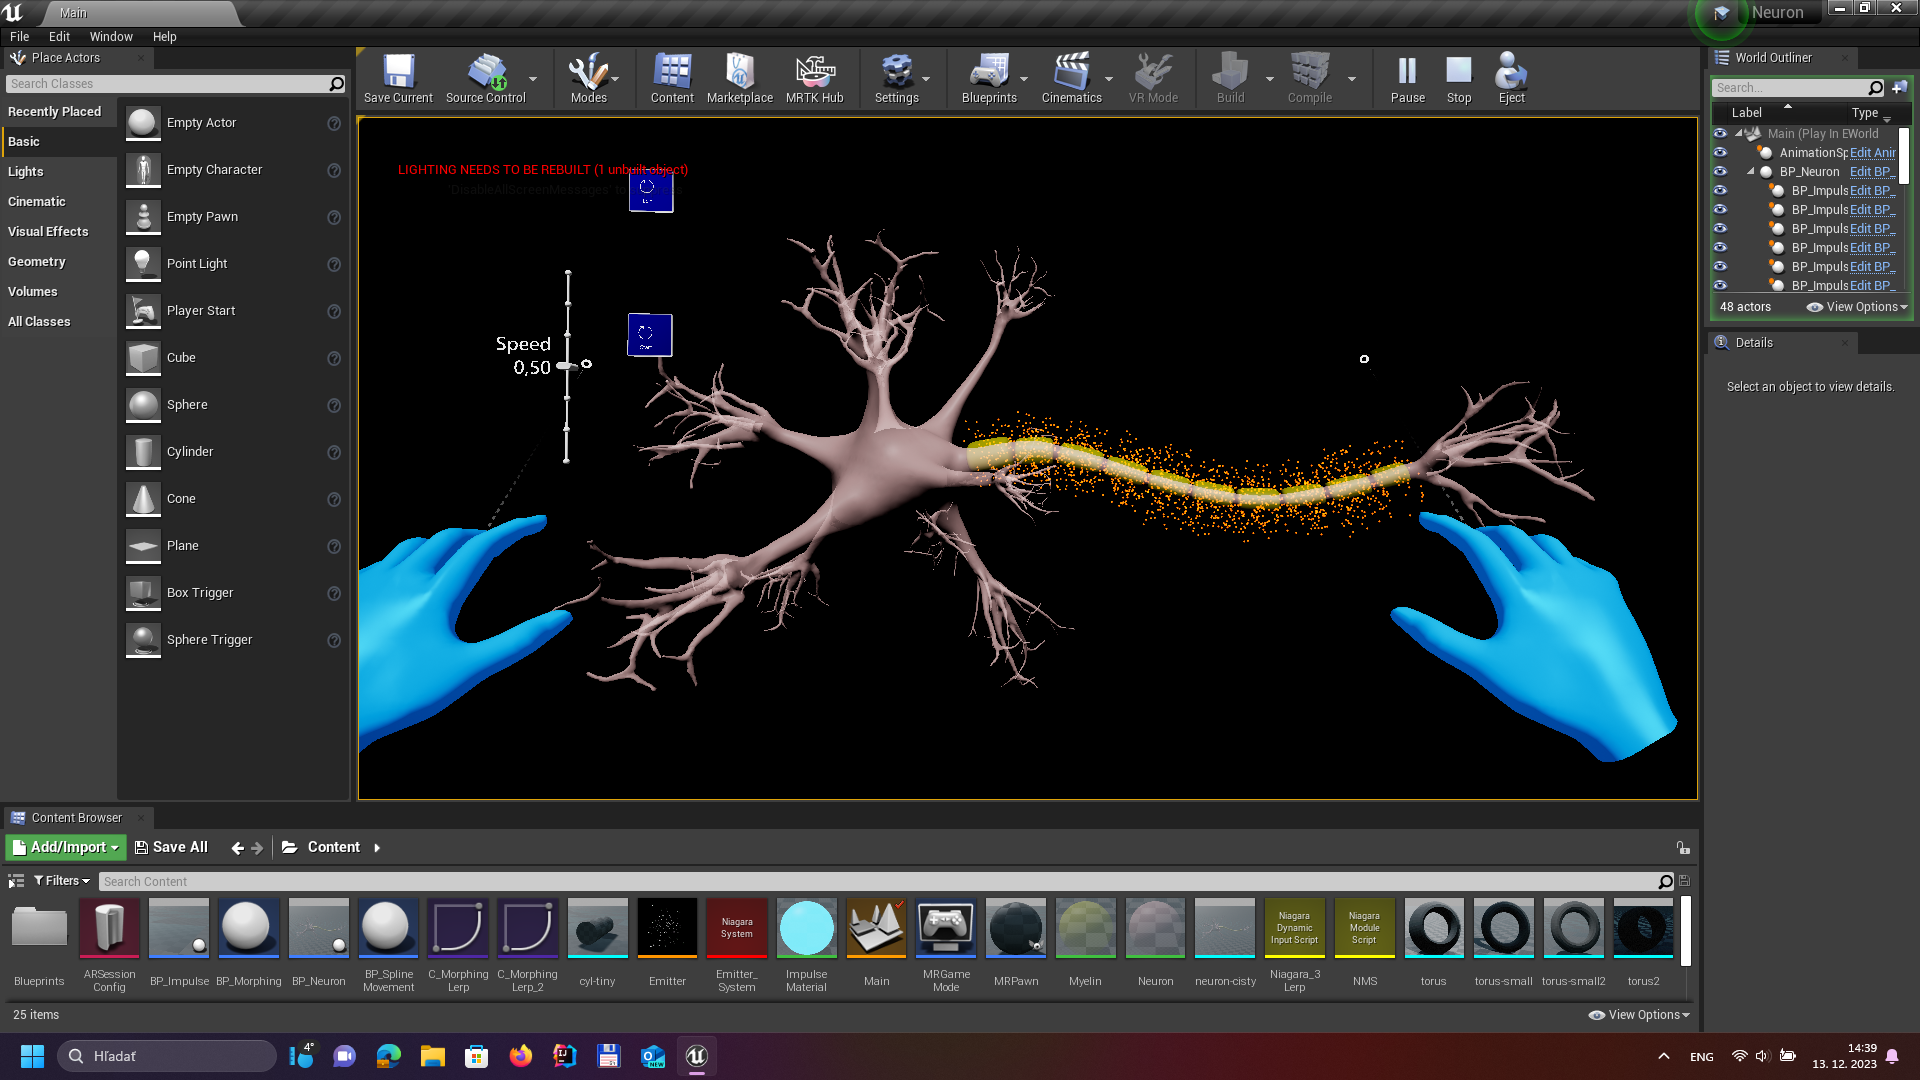
\includegraphics[width=11cm]{img/unreal.png}
    \end{center}
\end{frame}

\section{Didaktický výskum}
\begin{frame}{Didaktický výskum}
    \begin{itemize}
        \item Výskum prebehol na skupine 20 študentov ŠpMNDaG v Bratislave
        \item Kontrolnej skupine bol princíp nervového vzruchu sprístupnený bežnými didaktickými prostriedkami
        \item Vo výskumnej skupine bola použitá aplikácia
        \item Všetci študenti dostali dotazník
        \item Výsledky sa budú vyhodnocovať štatistickými metódami
    \end{itemize}    
\end{frame}
 
% \section{Stavba neurónu}
% \begin{frame}{Stavba neurónu}
    
% \end{frame}

% \section{Prenos nervového vzruchu}
% \begin{frame}{Prenos nervového vzruchu}
    
% \end{frame}

\section*{}
\begin{frame}{}
    Ďakujem za pozornosť.
\end{frame}

\end{document}